% !TEX encoding = UTF-8 Unicode
% !TEX TS-program = pdflatex
% !TEX spellcheck = en-US
% !TEX root = ../Report.tex

\chapter{Final Results}
Inside this chapter,we are going to show the results of our work, analizing the states evolution making a comparison between the Open and Cloosed loop condition, focusing on the different trajectories performed by the vehicle. In order to analyze the behaviour of our vehicle we set five different scenery that resumes most of the real driving condition. In particular we have analyzed the behaviour of the vehicle during a constant radios turn and a double turn that can be used as well to simulate a possible overtaking or an obstacles avoidance. Moreover, using a dedicated simroutine, we also analyzed the worst driving conditions relative to these scanery, taking into account possible drive disturbance as wind or bad road conditions. \\ 
Our controller provides a very precise response to the system variations, the value of the control action is generated taking into account the real time value of $\beta_{eq}$ and $\omega_{eq}$ as reference. The steady state condition are reached with a time in the order of few seconds. For our simulation we set a reference longitudinal speed of 90 km/h and a driver command steering angle of 120°. These value can be changed as wish in order to analize all the driving condition comprised in our speed and steering angle ranges; the overall simulation time is 60s. Regarging to the disturbance, we choiced to simulate the two main maneuvers (single and double turn) with the contribute of bad road condition as snow and ice, changing the relative fiction coefficient in the Simulik blocks, moreover we also make a simulation to consider environment contribute, in this case we fixed a lateral wind disturbance since as we know, it can modify the amount of aerodynamic forces of the car leading to unstable behaviour as well. All the disturbance hit the vehicle during the maneuver's initial turning phase.\\
\\
Analyzing these graphs is possible to see how the system try to reach the reference path and how the controller action improve the overall performance, it’s possible to appreciate a better behaviour in terms of stability, indeed the vehicle trajectory is more coherent with the ideal path. The car makes the manuever in a more safe and comfortable way, even in presence of environment  disturbances, avoiding over-under steering behaviour. The overall system maintain a proper robustness thanks to the optimal control algorithm. Using the vehicle dynamics toolbox is possible to get also the 3D rappresentation of the vehicle behaviour, altought these simulation require a lot of computational time. To conclude we can say that we achieved our desired value in terms of resonable angular speed and side slip angle, moreover a more detailed tuning phase of the Q and R matrix inside the cost function implementation can allow to further improve the overall performances.    

\begin{figure}[!h]
\section{Single turn}    
		\centering
	        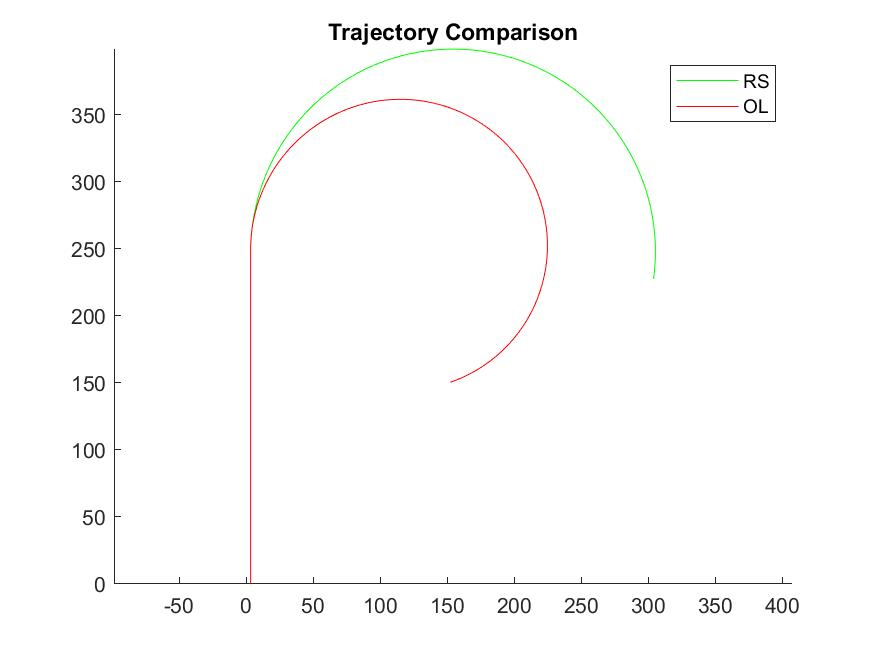
\includegraphics[scale=0.3]{./Images/ConstRadius/t} 
                \caption{(a)  RS vs OL comparison }
          
	\end{figure}

\begin{figure}[!h]
		\centering
	        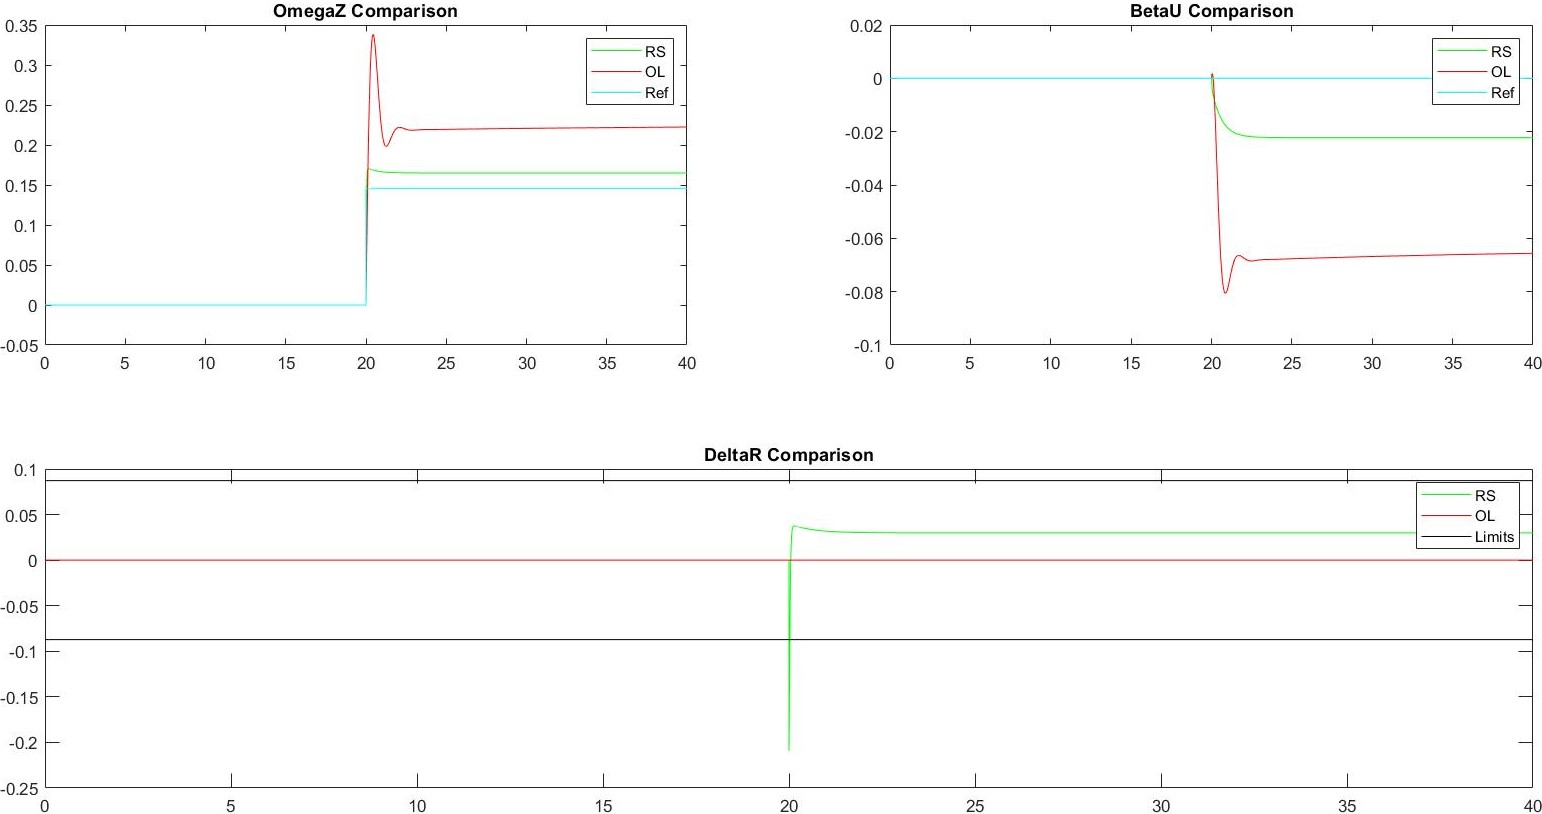
\includegraphics[scale=0.45]{./Images/ConstRadius/s} 
                \caption{(b)  Comparison of $\beta_{u}$, $\omega_{z}$ and $\delta_{r}$}
                \caption{Fig.1 Vehicle behaviour in constant radius scenario}
               
	\end{figure}

\begin{figure}[!h]
		\centering
	        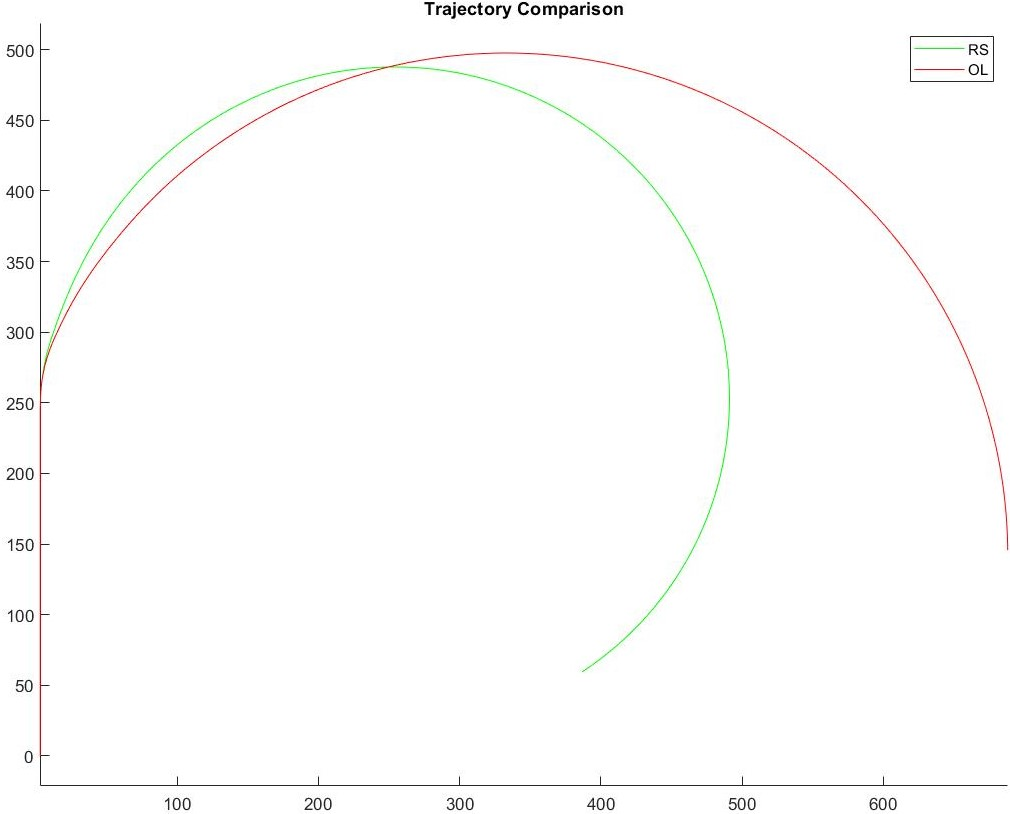
\includegraphics[scale=0.4]{./Images/ConstRSnow/t} 
                \caption{(a)  RS vs OL comparison}
          
	\end{figure}

\begin{figure}[!h]
		\centering
	        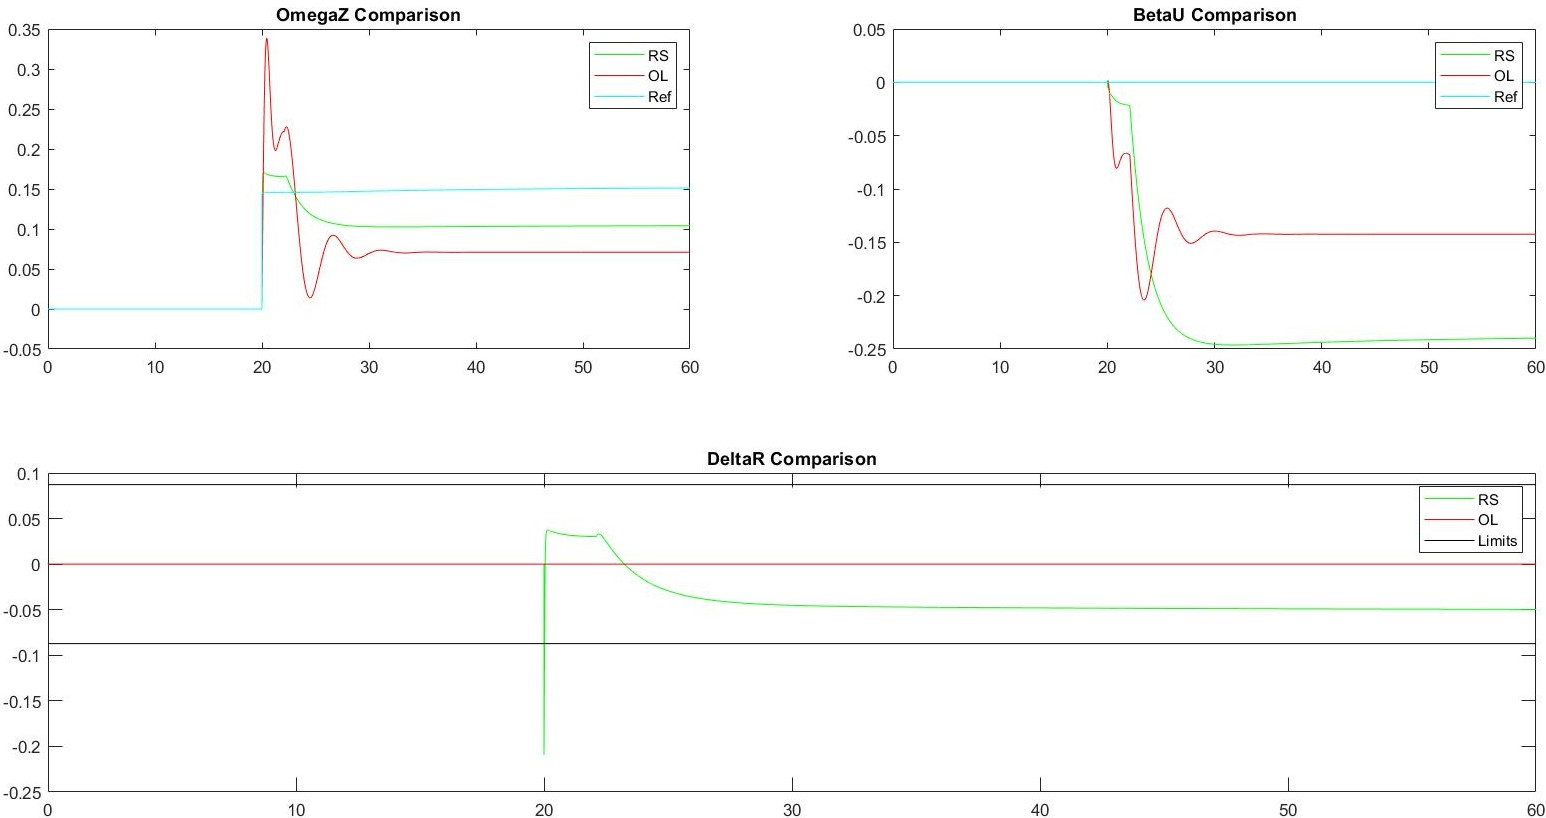
\includegraphics[scale=0.6]{./Images/ConstRSnow/s} 
                \caption{(b) Comparison of  $\beta_{u}$, $\omega_{z}$ and $\delta_{r}$}
                \caption{Fig.2 Constant Radius scenario with snow road}
               
	\end{figure}

\begin{figure}[!h]
		\centering
	        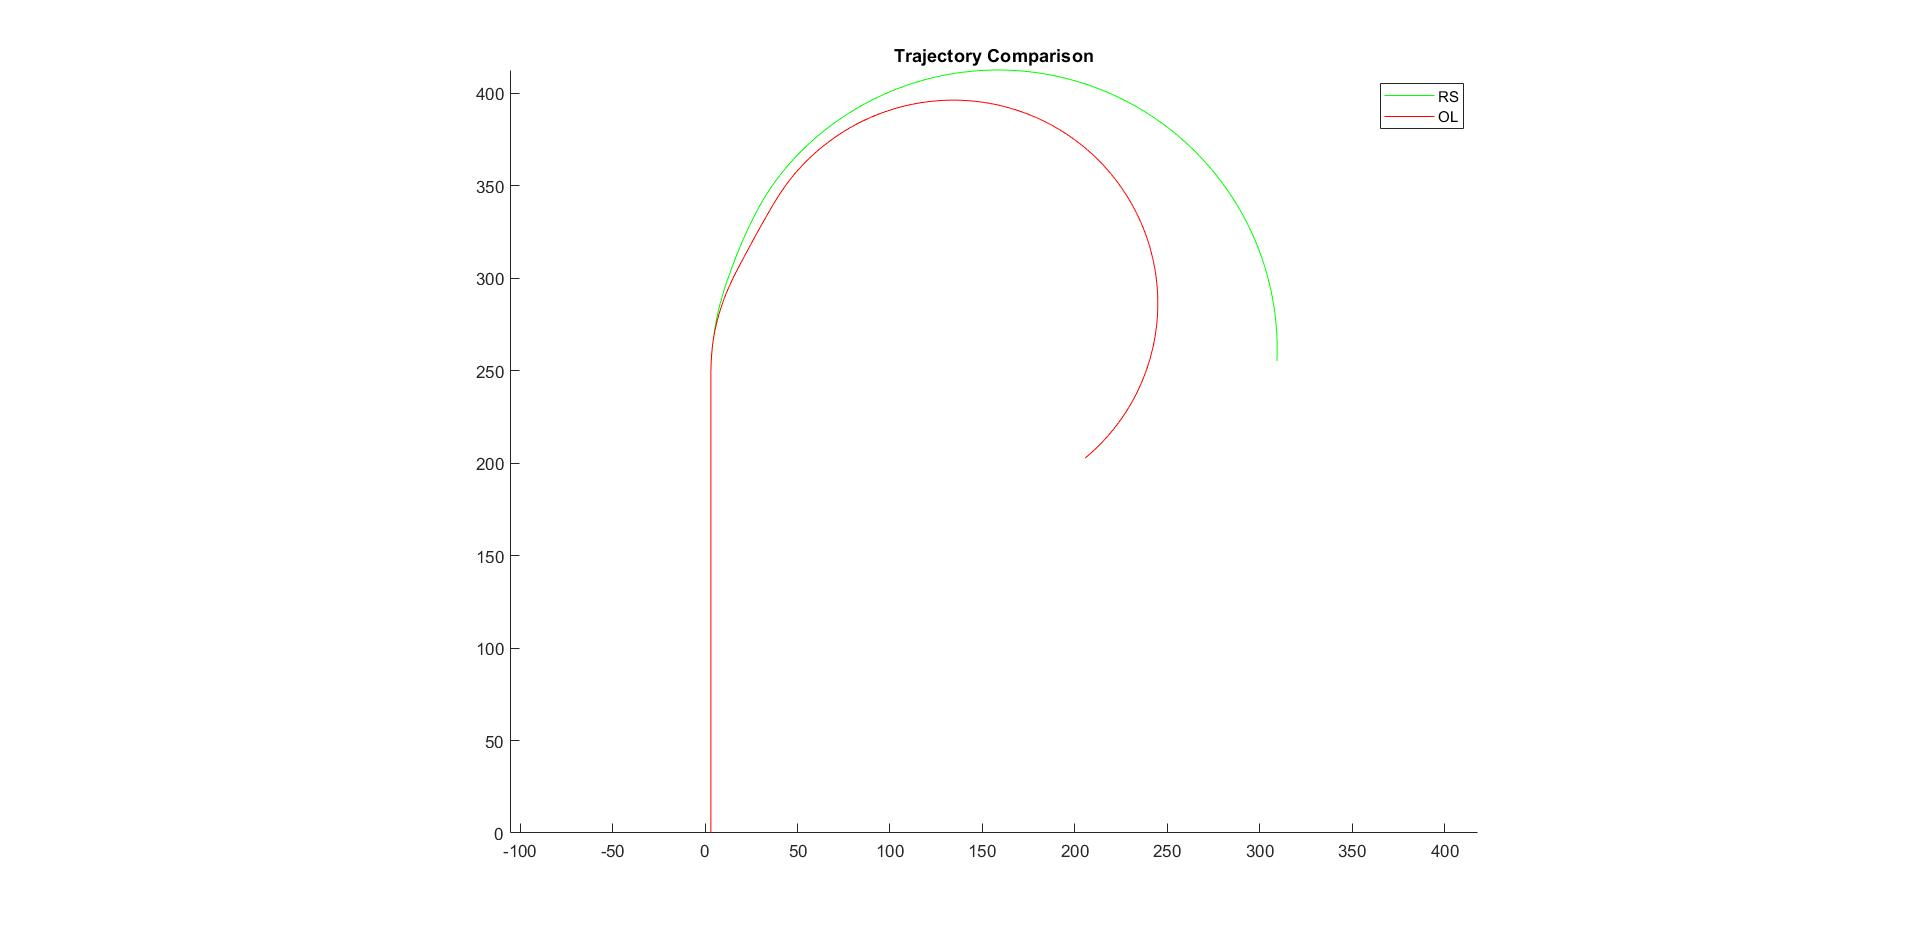
\includegraphics[scale=0.25]{./Images/ConstRwind/t} 
                \caption{(a)  RS vs OL comparison}
          
	\end{figure}

\begin{figure}[!h]
		\centering
	        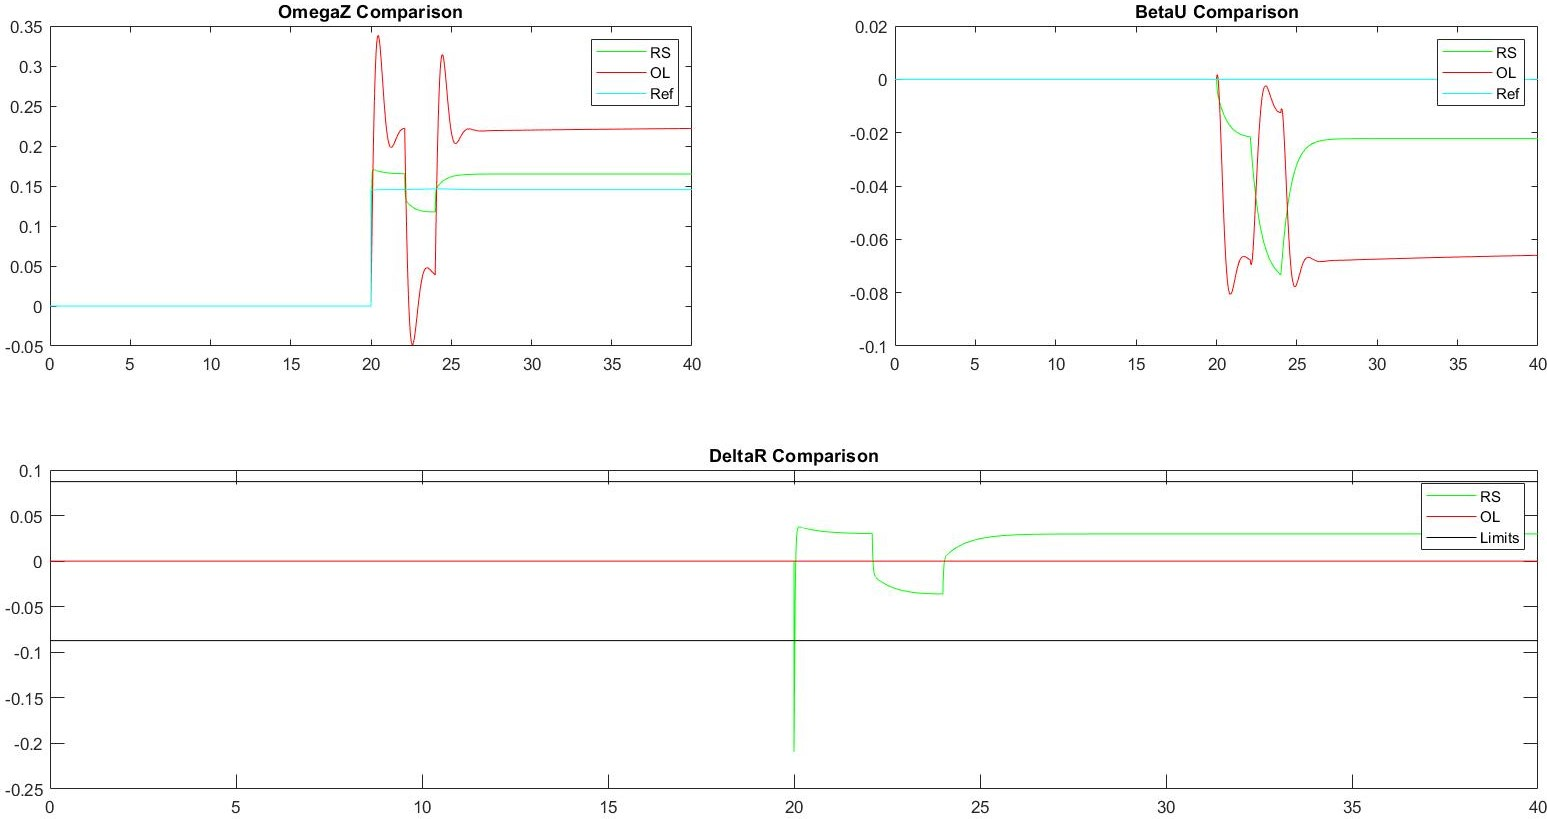
\includegraphics[scale=0.6]{./Images/ConstRwind/s} 
                \caption{(b) Comparison of  $\beta_{u}$, $\omega_{z}$ and $\delta_{r}$}
                \caption {Fig.3 Constant Radius scenario with lateral wind of 20 m/s}
	\end{figure}

\begin{figure}[!h]
\section{Double turn}
		\centering
	        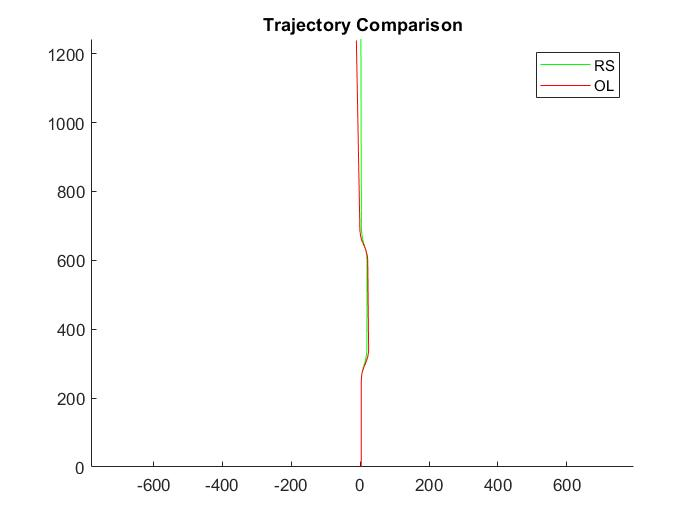
\includegraphics[scale=0.35]{./Images/LaneChange/t} 
                \caption{(a)  RS vs OL comparison}
             
	\end{figure}

\begin{figure}[!h]
		\centering
	        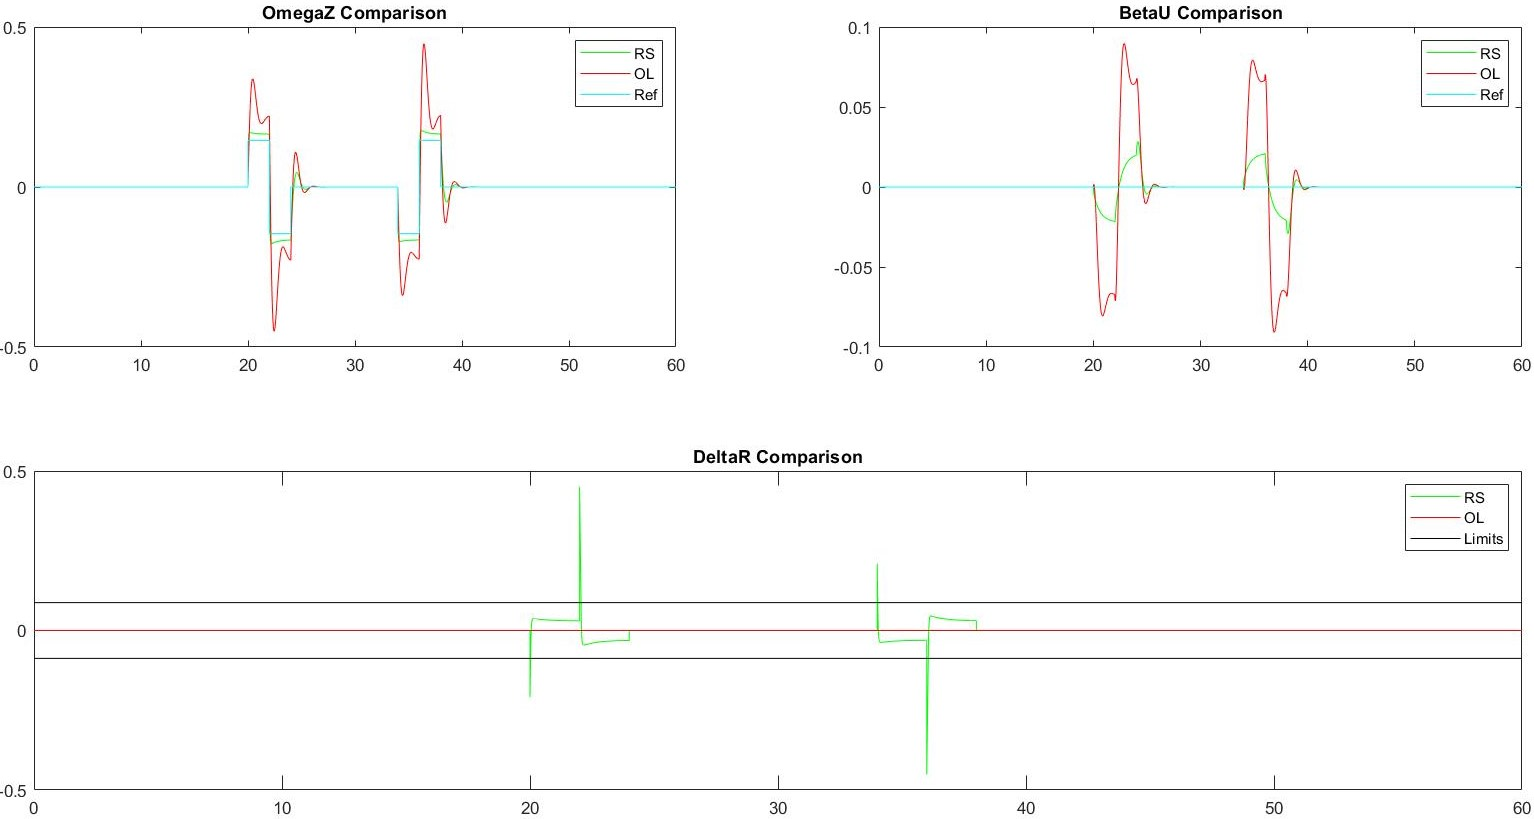
\includegraphics[scale=0.55]{./Images/LaneChange/s} 
                \caption{(b) Comparison of $\beta_{u}$, $\omega_{z}$ and $\delta_{r}$}
                \caption {Fig.4 Double turn witohut disturbance}
             
	\end{figure}

\begin{figure}[!h]
		\centering
	        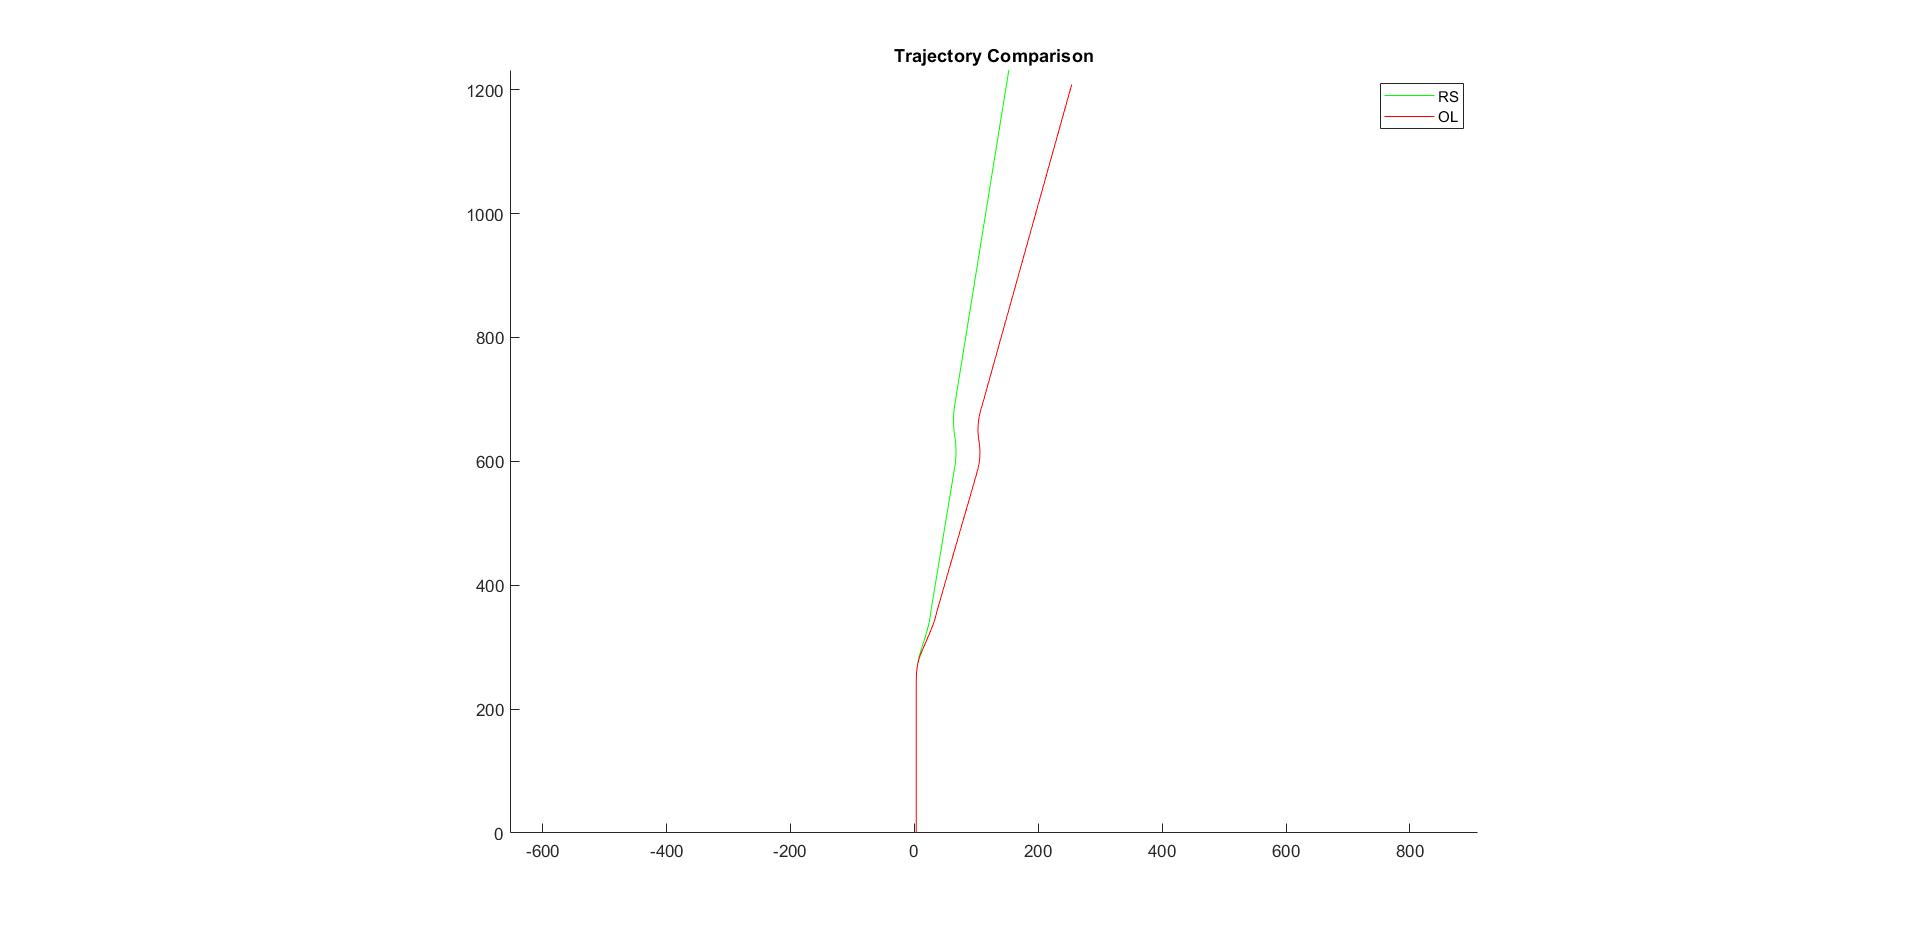
\includegraphics[scale=0.3]{./Images/LaneChangeIce/t} 
                \caption{(a)  RS vs OL comparison}
             
	\end{figure}

\begin{figure}[!h]
		\centering
	        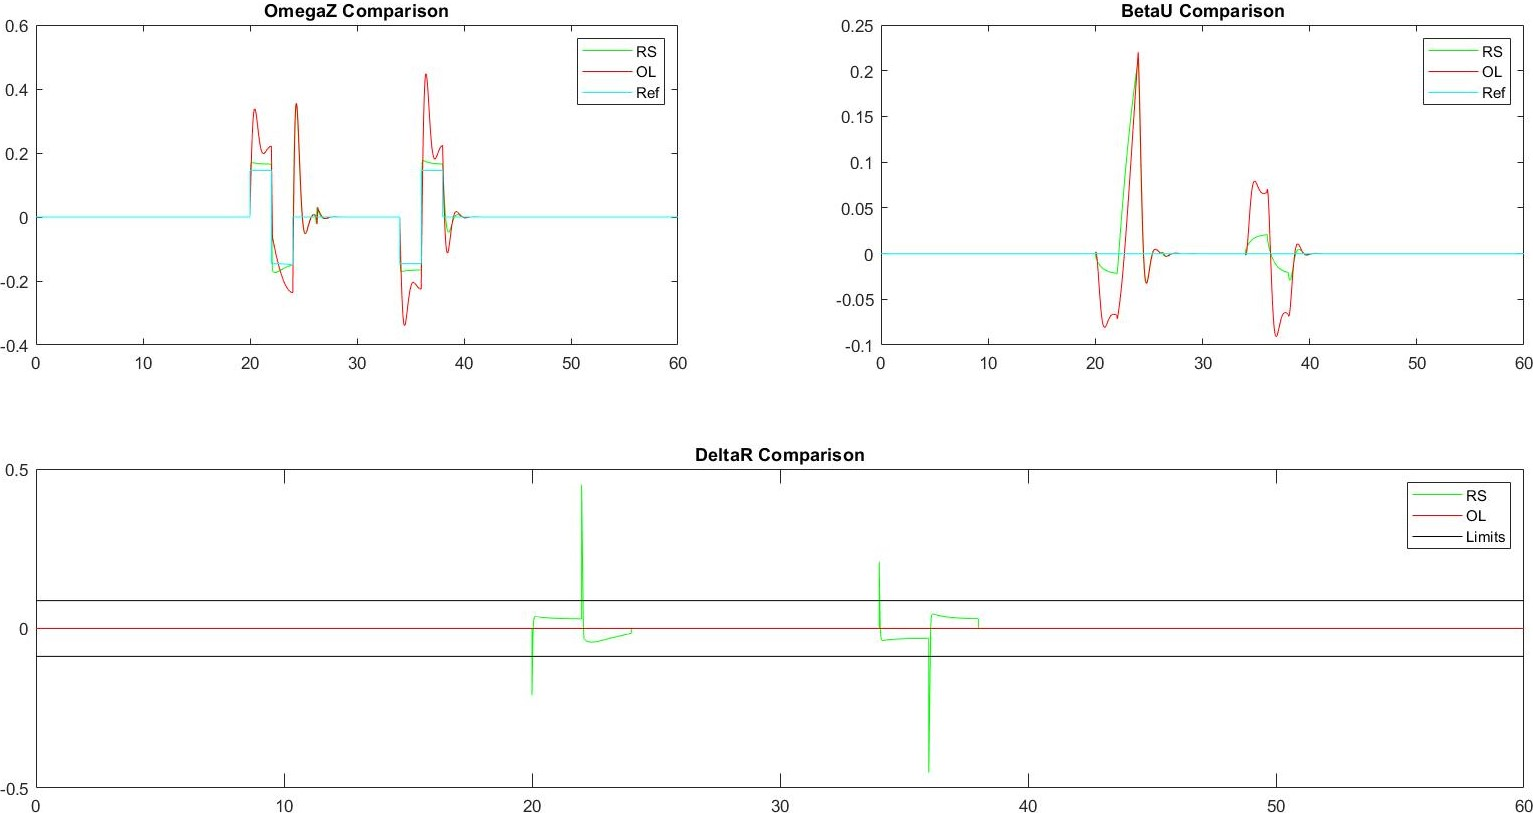
\includegraphics[scale=0.45]{./Images/LaneChangeIce/s} 
                \caption{(b) Comparison of $\beta_{u}$, $\omega_{z}$ and $\delta_{r}$} 
                \caption{Fig.5  Double turn in ice road}
        
 \end{figure}



    